\newpage
\section{Processes}
\subsection{Process Concept}
\subsubsection{Concept}
又称 jobs/tasks/process. Process是一个运行的实例. 

A process includes:
\begin{itemize}
    \item text section (code, 代码段)
    \item data section (global vars, 数据段)
    \item stack (function parameter, local vars, return addresses, 栈)
    \item heap (dynamically allocated memory, 堆)
\end{itemize}

heap增长需要 OS 操作, stack 是已分配的一块空间, 在其内增长, 超过触发 stack overflow. stack 与 heap 之间的区域称为 hole, 占据超过 90\% 的空间. 

\begin{figure}[!htb]
    \centering
    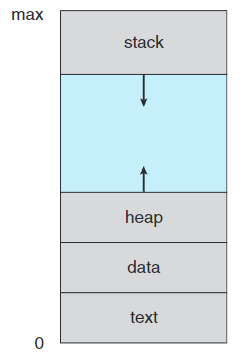
\includegraphics[width=0.22\textwidth]{pic/OS3/Layout of a process in memory.png}
    \caption{Layout of a process in memory}
\end{figure}

\subsubsection{Process State}
As a process executes, it changes state:
\begin{itemize}\small
    \item new: The process is being created
    \item running: Instructions are being executed
    \item waiting: The process is waiting/blocked for some event to occur
    \item ready (就绪): The process is waiting to be assigned to a processor
    \item terminated: The process has finished execution
\end{itemize}

\begin{figure}[!htb]
    \centering
    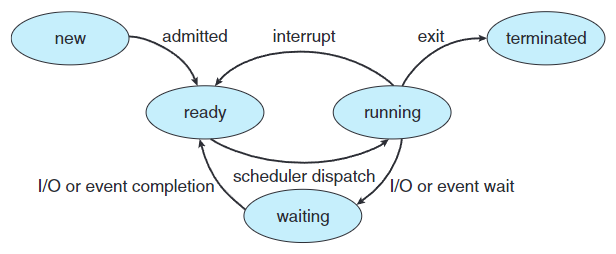
\includegraphics[width=0.42\textwidth]{pic/OS3/Diagram of process state.png}
    \caption{Diagram of process state transition}
\end{figure}


% \subsection{Process Scheduling}
% \subsection{Operations on Processes}
% \subsection{Cooperating Processes}
% \subsection{Interprocess Communication}
% \subsection{Communication in Client-Server Systems}